\input{../../headers/tdheaders.tex}

\section{Moto-réducteur}

Une étude dynamique permet de quantifier l'inertie totale $J_T$ rapportée sur l'axe d'un arbre moteur, de l'ensemble réducteur et moteur, ainsi que le coefficient de frottement visqueux total $f_T$. Le schéma fonctionnel de l'asservissement en vitesse du moteur suivi du réducteur est donné ci-dessous :

%\begin{figure}[!h]
%\begin{center}
%\begin{tikzpicture}[scale=1, every node/.style={scale=1}]
%\sbEntree{E}
%\sbComp{comp}{E}                
%\sbRelier[$C_v$]{E}{comp}
%\sbBloc{reg}{$\dfrac{K}{1+\tau.p}$}{comp}  
%\sbRelier[$\epsilon_v$]{comp}{reg}
%\sbComp{compdeux}{reg}
%\sbRelier[$U$]{reg}{compdeux}
%\sbBloc{res}{$\dfrac{1}{R}$}{compdeux}      
%\sbRelier[$\epsilon_U$]{compdeux}{res}
%\sbBloc{km}{$K_M$}{res} 
%\sbRelier[$I$]{res}{km}
%\sbSumh{comptrois}{km}
%\sbEntree{cp}
%\sbDecaleNoeudx[0]{comptrois}{cp}
%\sbDecaleNoeudy[-4]{comptrois}{cp}
%\sbRelier[$C_M$]{km}{comptrois}
%\sbRelier[$C_p$]{cp}{comptrois}
%\sbBloc{sys}{$\dfrac{\dfrac{1}{f_T}}{1+\dfrac{J_T}{f_T}.p}$}{comptrois} 
%\sbRelier[$C_U$]{comptrois}{sys}
%\sbBloc{rho}{$\rho$}{sys} 
%\sbRelier[$\Omega_M$]{sys}{rho}
%\sbSortie{S}{rho}
%\sbRelier[$\Omega_R$]{rho}{S}
%\sbDecaleNoeudy[7]{S}{U}
%\sbDecaleNoeudx[-20]{U}{V}
%\sbBlocr{cap}{$K_v$}{V}        
%\sbRelieryx{sys-rho}{cap}
%\sbRelierxy[$M_v$]{cap}{comp}
%\sbDecaleNoeudy[5]{S}{W}
%\sbDecaleNoeudx[-8]{W}{X}
%\sbBlocr{ke}{$K_E$}{X}        
%\sbRelieryx{sys-rho}{ke}
%\sbRelierxy[$M_U$]{ke}{compdeux}
%\end{tikzpicture}
%\end{center}
% \caption{Schéma bloc}
% \label{blocs1}
%\end{figure}

\begin{figure}[!h]
\begin{center}
\begin{tikzpicture}[scale=1, every node/.style={scale=1}]
\sbEntree{E}
\sbBloc{kv}{$K_a$}{E}
\sbRelier[$\Omega_c$]{E}{kv}
\sbComp{comp}{kv} 
\sbRelier[$C_v$]{kv}{comp}
\sbBloc{reg}{$\dfrac{K}{1+\tau.p}$}{comp}  
\sbRelier[$\epsilon_v$]{comp}{reg}
\sbComp{compdeux}{reg}
\sbRelier[$U$]{reg}{compdeux}
\sbBloc{res}{$\dfrac{1}{R}$}{compdeux}      
\sbRelier[$\epsilon_U$]{compdeux}{res}
\sbBloc{km}{$K_M$}{res} 
\sbRelier[$I$]{res}{km}
\sbSumh{comptrois}{km}
\sbEntree{cp}
\sbDecaleNoeudx[0]{comptrois}{cp}
\sbDecaleNoeudy[-4]{comptrois}{cp}
\sbRelier[$C_M$]{km}{comptrois}
\sbRelier[$C_p$]{cp}{comptrois}
\sbBloc{sys}{$\dfrac{\dfrac{1}{f_T}}{1+\dfrac{J_T}{f_T}.p}$}{comptrois} 
\sbRelier[$C_U$]{comptrois}{sys}
\sbBloc{rho}{$\rho$}{sys} 
\sbRelier[$\Omega_M$]{sys}{rho}
\sbSortie{S}{rho}
\sbRelier[$\Omega_R$]{rho}{S}
\sbDecaleNoeudy[7]{S}{U}
\sbDecaleNoeudx[-20]{U}{V}
\sbBlocr{cap}{$K_v$}{V}        
\sbRelieryx{sys-rho}{cap}
\sbRelierxy[$M_v$]{cap}{comp}
\sbDecaleNoeudy[5]{S}{W}
\sbDecaleNoeudx[-8]{W}{X}
\sbBlocr{ke}{$K_E$}{X}        
\sbRelieryx{sys-rho}{ke}
\sbRelierxy[$M_U$]{ke}{compdeux}
\end{tikzpicture}
\end{center}
 \caption{Schéma bloc}
 \label{blocs1}
\end{figure}


Caractéristiques du moteur électrique :
\begin{itemize}
 \item constante de la fcem : $K_E=0,6 V.s.rad^{-1}$,
 \item constante de couple : $K_M=0,7 N.m.A^{-1}$,
 \item résistance rotorique : $R = 4,5 \Omega$,
 \item inductance L négligée.
\end{itemize}

Données :
\begin{itemize}
 \item $J_T=2,8kg.m^2$, $f_T=1,5.10^{-3}N.m.s.rad^{-1}$,
 \item $K=200$,
 \item $K_V=0,01V.tr^{-1}.min$,
 \item $\tau=15ms$,
 \item $\rho=0,7$,
 \item $C_V(t)$ est la tension de consigne de vitesse, $\epsilon_V(t)$ l'écart de vitesse, $m_V(t)$ la mesure de vitesse
 \item $u(t)$ est la tension de commande, $U(t)$ l'écart de tension, $m_U(t)$ la mesure de tension,
 \item $C_M(t)$ est le couple moteur, $c_U(t)$ le couple utile, $c_P(t)$ le couple dû aux perturbations,
 \item $\Omega_M(t)$ est la vitesse de rotation du moteur, $\Omega_R(t)$ la vitesse de rotation du rouleau.
\end{itemize}

\paragraph{Question 1 :} En supposant qu'il n'y ait pas de perturbation ($C_P(t)$ est nul), donner l'expression de la fonction de transfert : $H_1(p)=\frac{\Omega_M(p)}{U(p)}_{C(p)=0}$

Préciser littéralement et numériquement, le gain $K_1$ et la constante de temps $\tau_1$.

~\

Nous nous intéressons maintenant à la boucle d'asservissement en vitesse d'entrée $\Omega_C(p)$ et de sortie $\Omega_M(p)$.

\paragraph{Question 2 :} En supposant toujours que $C_P(t)$ est nul, déterminer littéralement la fonction de transfert en boucle ouverte : $G_2(p)=\frac{M_V(p)}{\epsilon_V(p)}$	

\paragraph{Question 3 :} Déterminer $\epsilon_V(p)$ en fonction de $C_V(p)$ et $G_2(p)$. Puis en déduire l'écart statique
$ \displaystyle \epsilon_{Vs}=\epsilon_V(+\infty)=\lim_{t\rightarrow + \infty}\epsilon_V(t)$ pour $C_V(p)$ un échelon unitaire. Déterminer $K_a$ pour que l'écart statique soit nul lorsque $\Omega_c(p)=\Omega_R(p)$. Faire une application numérique pour $\epsilon_{Vs}$ dans le cas où $C_V(t)$ est un échelon unitaire.

\paragraph{Question 4 :} En supposant toujours que $C_P(t)$ est nul, en déduire littéralement la fonction de transfert en boucle fermée : $H_2(p)=\frac{\Omega_M(p)}{\Omega_c(p)}$	

\paragraph{Question 5 :} Montrer que l'on peut assimiler la fonction du transfert $H_2(p)$ à une fonctions $H'_2(p)$ du premier ordre, déterminer son temps de réponse.

\paragraph{Question 6 :} On donne ci-dessous, la réponse indicielle du système, à une entrée de type échelon unitaire $(C_V(t)=1V)$. Placer sur la figure le temps de réponse à 5\%. Donner les valeurs numériques correspondantes et retrouver le résultat de la question précédente.

\begin{figure}[!h]
 \centering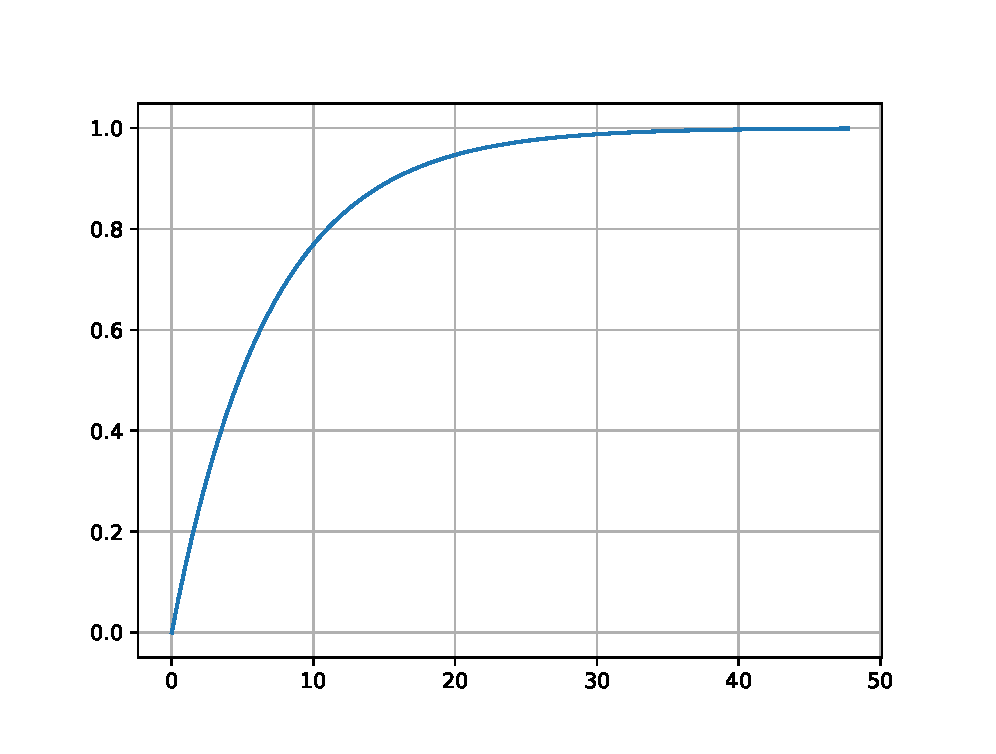
\includegraphics[width=0.6\linewidth]{img/motoreduc_courbe}
 \caption{Réponse indicielle}
 \label{bloc2}
\end{figure}

~\

\newpage

\section{Diravi}

L'objectif est de compléter le schéma bloc de la Diravi. En effet, lors de la précédente étude du système Diravi, un certain nombre d'équation dans le domaine de Laplace ont été mises en évidence. L'angle $\alpha_{volant}$ doit être exprimé en radian.

\begin{minipage}{0.49\linewidth}
Équations dans le domaine de Laplace:
\begin{itemize}
 \item $Q(p)=k.X(p)$,
 \item $Q(p)=S.p.Y(p)+Q_p(p)+Q_c(p)$,
 \item $Q_c(p)=\dfrac{V}{2}.\beta.p.\Delta_p(p)$,
 \item $Q_p(p)=f.\Delta_p(p)$,
 \item $F(p)=S.\Delta_p(p)$,
 \item $F(p)=M.p^2.Y(p)$.
\end{itemize}
\end{minipage}\hfill
\begin{minipage}{0.49\linewidth}
Données numériques:
\begin{itemize}
 \item $K_a=\dfrac{34}{57}$,
 \item $K_b=0,04mm.\degree^{-1}$,
 \item $K_c=\dfrac{1}{500}tr.mm^{-1}$,
 \item $K_d=K_a$,
 \item $k=0,24m^3.s^{-1}.mm^{-1}$,
 \item $S=3000mm^2$,
 \item $M=500kg$,
 \item $f=6.dm^3.min^{-1}.MPa^{-1}$,
 \item $\dfrac{V.\beta}{2}=2.10^{-5}.dm^3.MPa^{-1}$
\end{itemize}
\end{minipage}

Ces résultats vont servir à compléter les blocs vides du schéma bloc de la Diravi.

\begin{figure}[!h]
\begin{center}
\begin{tikzpicture}[scale=1, every node/.style={scale=1}]
\sbEntree{E}
\sbBloc{ka}{$K_a$}{E}
\sbRelier[$\alpha_{vol}$]{E}{ka}
\sbComp{comp}{ka}                
\sbRelier[$\alpha$]{ka}{comp}
\sbBloc{reg}{$K_b$}{comp}  
\sbRelier[$\epsilon$]{comp}{reg}
\sbBloc{k}{}{reg}  
\sbRelier[$X(p)$]{reg}{k}
\sbComp{compdeux}{k}
\sbRelier[$Q(p)$]{k}{compdeux}
\sbDecaleNoeudx[8]{compdeux}{re}
\sbBloc{res}{}{re}      
\sbRelier[$\epsilon_Q$]{compdeux}{res}
\sbDecaleNoeudx[13]{res}{r}
\sbSortie{S}{r}
\sbRelier[$Y(p)$]{res}{S}
\sbDecaleNoeudy[5]{S}{U}
\sbDecaleNoeudx[-5]{U}{V}
\sbBlocr{cap}{}{V}        
\sbRelieryx{res-S}{cap}
\sbBlocr{pis}{$\dfrac{1}{S}$}{cap}
\sbRelier[$F(p)$]{cap}{pis}
\sbBlocr{beta}{}{pis}
\sbRelier[$\Delta_p(p)$]{pis}{beta}
\sbDecaleNoeudx[-10]{beta}{c}
\sbCompSum{comptrois}{c}{}{+}{}{+}
\sbRelier[$Q_c(p)$]{beta}{comptrois}
\sbRelierxy[$M_v$]{comptrois}{compdeux}
\sbDecaleNoeudy[4]{pis}{G}
\sbDecaleNoeudx[-2]{G}{fe}
\sbBlocr{f}{}{fe}
\sbRelierxy[$Q_p(p)$]{f}{comptrois}
\sbRelieryx{pis-beta}{f}
\sbDecaleNoeudy[13]{S}{W}
\sbDecaleNoeudx[-8]{W}{X}
\sbBlocr[5]{kc}{$K_c$}{X}        
\sbRelieryx{res-S}{kc}
\sbBlocr[5]{kd}{$K_d$}{kc} 
\sbRelier[$\alpha_{pignon}$]{kc}{kd}  
\sbRelierxy[$\alpha'$]{kd}{comp}
\end{tikzpicture}
\end{center}
 \caption{Schéma bloc}
 \label{blocs1}
\end{figure}

\paragraph{Question 1:} Compléter le schéma bloc.

\paragraph{Question 2:} Déterminer $FTBO(p)=\dfrac{\alpha'(p)}{\epsilon(p)}$ et $FTBF(p)=\dfrac{Y(p)}{\alpha_{vol}(p)}$ du système.

\paragraph{Question 3:} Donner les caractéristiques de la FTBF.

\paragraph{Question 4:} Exprimer toutes les constantes dans des unités S.I. de base sauf le Newton qu'il est conseillé de conserver.

\paragraph{Question 5:} Montrer qu'il est possible de simplifier la FTBF, donner alors les expressions littérales puis les valeurs numériques de ces caractéristiques.

\paragraph{Question 6:} Déterminer le temps de réponse à 5\% et le dépassement D\%.

\section{Centre usinage grande vitesse}

\subsection{Présentation du système}

La société PCI conçoit et réalise des centres d'Usinage Grande Vitesse ainsi que des machines spéciales de production.

\begin{minipage}{0.48\linewidth}
 \centering 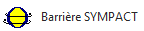
\includegraphics[width=0.6\linewidth]{img/img01}
\end{minipage}\hfill
\begin{minipage}{0.48\linewidth}
 \centering 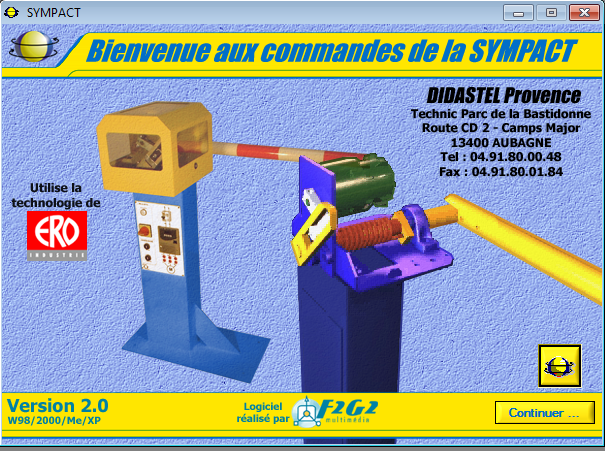
\includegraphics[width=0.6\linewidth]{img/img02}
\end{minipage}

La principale caractéristique d'une structure parallèle réside dans le fait que la mise en mouvement de l'organe mobile sur un axe ne demande pas la mise en mouvement des actionneurs et dispositifs cinématiques nécessaires à la mise en mouvement des autres organes mobiles sur les autres axes. Ainsi, la structure parallèle adopte une cinématique assurant le positionnement et le déplacement de chaque partie mobile par rapport au bâti fixe.

La partie fixe de chaque actionneur est solidaire de l'élément fixe, la partie mobile de chaque actionneur étant solidaire de l'organe mobile par l'intermédiaire d'un élément de liaison.

\begin{center}
 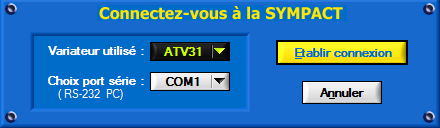
\includegraphics[width=0.3\linewidth]{img/img05}
\end{center}

Un des inconvénients d'une telle structure réside dans la multiplication des articulations dont une des conséquences est le maintien en position précis de la broche à l'extrémité des bras de positionnement (Figure 4). Cela crée un bras de levier important par rapport à la base des bras de positionnement difficilement paramétrable. La solution à ce problème de bras de levier a été jusqu'à maintenant de placer l'axe de la broche verticalement afin que les effets de la gravité soient moindres.

%Le système:

Le sujet se propose d'étudier plus particulièrement un des bras de la machine au travers de trois fonctions techniques de cette machine-outil : la gestion de l'arrêt d'urgence, la gestion de la vitesse d'avance et le suivi de trajectoire.

%Dans cette étude on se propose :
%\begin{itemize}
% \item D'étudier l'architecture d'ensemble de la machine,
% \item D'étudier la robustesse de la fonction arrêt d'urgence,
% \item D'analyser l'obtention d'une vitesse d'avance de l'outil et la commande d'un axe de la machine-outil pour atteindre cette vitesse d'avance,
% \item D'analyser la commande en position d'un axe de la machine-outil.
%\end{itemize}

\newpage

\subsection{Modélisation de l'Axe 1 : Boucle de couple}

Un schéma simplifié du système asservi de l'axe est le suivant:

\begin{center}
 \includegraphics[width=0.8\linewidth]{img/img18}
\end{center}

Simplification, hypothèses :

On considère de faibles déplacements autour d'une position de référence. Le comportement de l'Axe1 de la MOCN (Machine Outil à Commande Numérique) Triptéor peut-être considéré comme linéaire.

%Le filtre de consigne de couple est désactivé (équivalent à un gain unitaire).

Notation :
\begin{itemize}
 \item $x_{ref}(t)$ : référence de position fournie par l'interpolateur de la CN 840D,
 \item $x(t)$ : position de l'Axe1,
 \item $\Omega_{ref}(t)$ : référence de vitesse angulaire de la MSAP (Machine Synchrone AutoPilotée) de l'Axe1.
 \item $\Omega(t)$ : vitesse angulaire de la MSAP de l'Axe1.
 \item $c_{ref}(t)$ : référence de couple fournie par la CN 840D au variateur de la MSAP de l'Axe1.
 \item $c(t)$ : image du couple fourni par la MSAP de l'Axe1.
\end{itemize}

Chaque axe de la MOCN est piloté par son variateur. Ceux-ci possèdent une boucle interne de courant. Ceci permet de gérer, au plus près de l'axe, deux grandeurs essentielles :
\begin{itemize}
 \item Le couple fourni par la MSAP (le couple est linéairement lié au courant, c'est d'ailleurs cette valeur qui est retournée par l'IHM (Interface Homme Machine) de la CN 840D),
 \item L'état thermique de la MSAP (les pertes joules responsables de l'échauffement de la MSAP sont de la forme $r.I_{rms}^2$ ($r$ la résistance et $I_{rms}$ la valeur efficace des courants dans les enroulements de la MSAP)).
\end{itemize}

Le réglage de cette boucle interne conditionne complètement les dynamiques des autres boucles externes (vitesse, position) : Les boucles externes ne peuvent bien évidemment pas être plus rapides que cette boucle interne.

%La CN 840D possède des outils d'aide aux réglages des différentes boucles d'asservissement présent dans une MOCN.

%Cette CN étant bien sur numérique le signal est échantillonné.

%Le pas de calcul est de $125\mu s$, durée très faible devant la dynamique des différentes variables utilisées dans ce sujet. On considèrera donc que les variables sont assimilables à des variables continues du temps.

On a fait subir, après avoir réglé la boucle de couple, une réponse à l'échelon de référence de couple (Figure 17) de quelques \% du couple nominal (valeur faible afin de limiter les effets des non-linéarités).

Le temps est exprimé en millisecondes.

\begin{center}
 \includegraphics[width=0.7\linewidth]{img/img19}
\end{center}

Cette réponse fait apparaître un retard dans la réponse en couple.

Afin d'augmenter la lisibilité de l'essai réalisé sous la CN 840D nous avons retravaillé les courbes sous un outil de simulation.

Dans une première partie nous ferons abstraction de ce retard.

Le résultat de la réponse à un échelon de la boucle de couple sans prise en compte du retard est donné.

\begin{center}
 \includegraphics[width=0.8\linewidth]{img/img20}
\end{center}

\paragraph{Question 1:} Par analyse de la réponse en couple à l'échelon d'amplitude 3, donner la transmittance type 1er ordre sous forme canonique reliant le couple de sortie $C(p)$ au couple de référence $C_{ref}(p)$. On précisera sur la figure les tracés nécessaires à l'obtention de cette transmittance.

Prise en compte du retard. Le résultat de la réponse à un échelon de la boucle de couple avec prise en compte du retard est donné.

\begin{center}
 \includegraphics[width=0.8\linewidth]{img/img21}
\end{center}

\paragraph{Question 2:} Par analyse de la réponse en couple à l'échelon d'amplitude trois avec prise en compte du retard et en reprenant la transmittance de la question 1, donner la transmittance type 1er ordre avec retard sous forme canonique reliant le couple de sortie $C(p)$ au couple de référence $C_{ref}(p)$. On précisera sur la figure les tracés nécessaires à l'obtention de cette transmittance.

La transmittance obtenue avec prise en compte du retard est non-linéaire.

Par approximation, on cherche à linéariser cette transmittance.

\paragraph{Question 3:} Remplacer la fonction retard pur par son développement limité à l'ordre 1: $(e^x\simeq 1+x)$. Donner la fonction de transfert approximée de la boucle de couple $\dfrac{C(p)}{C_{ref}(p)}$ faisant apparaître un deuxième pôle stable.

Montrer que le résultat peut se mettre sous la forme :

$\dfrac{C(p)}{C_{ref}(p)}=\dfrac{0.97}{(1+0.00025.p)(1+0.00015.p)}$

\iffalse

\paragraph{Question 4:} Tracer le diagramme de Bode asymptotique en gain et en phase de la fonction de transfert linéarisée
$\dfrac{C(p)}{C_{ref}(p)}=\dfrac{0.97}{(1+0.00025.p)(1+0.00015.p)}$ en fonction de la pulsation $\omega$ ($rad.s^{-1})$. On précisera sur le diagramme les pentes, le gain statique (sous la forme 20log(cste)) et les valeurs des phases.

Un essai en régime harmonique sur le Triptéor de la boucle de couple a donné le diagramme de Bode en phase de la figure.

\begin{center}
 \includegraphics[width=0.8\linewidth]{img/img22}
\end{center}

Nota : Le résultat de l'analyse harmonique fourni par la C.N. 840D est compris entre +/- 180°.

La phase réelle comprise entre 2kHz et 4kHz est bien sur comprise entre -180° et -360°.

La phase est fournie en fonction de la fréquence f (Hz).

\paragraph{Question 5:} L'évolution de la phase obtenue ci-dessus est-elle identique à celle du diagramme de Bode obtenue à la question 4 ? Argumenter votre réponse.

\fi

\newpage

\section{Système de traite automatique des vaches}

\subsection{Présentation du système}

Les agriculteurs, producteurs laitiers, sont soumis à des réglementations strictes quant à la production du lait, en terme de respect de l'environnement, de mesures d'hygiène et de qualité de vie des animaux. Traire les vaches est une opération pénible et répétitive. Cette opération doit se faire dans le respect des animaux et elle est soumise à des horaires contraignants.

Le robot à étudier améliore de façon notable la santé et la qualité de vie des producteurs laitiers, tout en préservant le rythme des animaux et en garantissant la qualité du lait. Il assure à la fois la traite des vaches, leur alimentation et le contrôle de la qualité du lait.

\subsection{Description du robot de traite}

\begin{minipage}{0.48\linewidth}
 \centering \includegraphics[width=0.75\linewidth]{img/img01v}
\end{minipage}\hfill
\begin{minipage}{0.48\linewidth}
 \centering \includegraphics[width=0.75\linewidth]{img/img02v}
\end{minipage}

~\

Le robot est composé:
\begin{itemize}
 \item d'une zone (box où la vache est installée lors de la traite) composée d'une structure tubulaire mécano-soudée, équipée de 2 portes (entrée et sortie), d'un tapis de pesée et d'une auge réservée à l'alimentation solide (granulés),
 \item d'un système de bras articulé, permettant au système de traite de se positionner au mieux pour traire la vache,
 \item d'une interface homme/machine, écran de contrôle tactile, qui permet au personnel agricole d'obtenir des renseignements sur le processus en cours et de gérer d'éventuelles opérations de maintenance.
\end{itemize}

\begin{center}
 \includegraphics[width=0.7\linewidth]{img/traite_bdd}
\end{center}

\begin{center}
 \includegraphics[width=0.8\linewidth]{img/traite_req}
\end{center}

~\

Le système de traite étant positionné suivant $\overrightarrow{y_0}$ et suivant $\overrightarrow{z_0}$, nous allons nous intéresser plus particulièrement au mouvement du chariot 1, suivant la direction $\overrightarrow{x_0}$, lorsque le robot est en phase de traite de la vache (gobelets trayeurs positionnés sur la vache et en mode extraction du lait).

\newpage

Structure de l'axe motorisé du chariot :

\begin{center}
 \includegraphics[width=0.8\linewidth]{img/img118}
\end{center}

Chaîne d'énergie :
\begin{itemize}
 \item modulateur d'énergie:
 \begin{itemize}
  \item gain $K_a=6$.
 \end{itemize}
 \item moteur CC:
  \begin{itemize}
  \item résistance de l'induit: $R=0,56\Omega$,
  \item inductance: $L=0,0053 H$,
  \item constante de fem: $K_e=0,8V.s.rad^{-1}$,
  \item constante de couple $K_i=0,8N.m.A^{-1}$.
 \end{itemize}
 \item réducteur :
  \begin{itemize}
  \item réduction $r=\Omega_m/\Omega_r=19$.
  \end{itemize}
 \item pignon-crémaillère:
  \begin{itemize}
  \item diamètre du pignon : $\Phi_p=50mm$.
  \end{itemize}
 \item dynamique du chariot 1 dans son mouvement par rapport au bâti :
  \begin{itemize}
  \item $F(t)-F_p(t)=M_{eq}.\Gamma_{(chariot 1/bati)}$,
  \item $F(t)$ est l'effort transmis pour le déplacement du chariot (en $N$),
  \item $F_p(t)$ est un effort qui représente la perturbation que peut subir le système (en $N$),
  \item masse équivalente (en déplacement) : $M_{eq}=50kg$,
  \item $\Gamma_{(chariot 1/bati)}$ est l'accélération du chariot par rapport au bâti (en $m.s^{-2}$).
  \end{itemize}
\end{itemize}

~\

Chaîne d'information :
\begin{itemize}
 \item codeur absolu et CNA: $K_c=0,055V/mm$.
\end{itemize}

~\

La modélisation (schéma-bloc du déplacement du chariot en translation par rapport au bâti) est donnée sur le schéma suivant. 

\begin{center}
 \includegraphics[width=\linewidth]{img/img119}
\end{center}

\newpage 

Hypothèses de travail :
\begin{itemize}
 \item il n'y a pas de perturbation extérieure, donc $F_p(p)=0$,
 \item la valeur du correcteur est $C(p)=1$.
\end{itemize}

~\

\textit{Vous allez tout d'abord modéliser le comportement du moteur à courant continu.}

\paragraph{Question 1:} Déterminer la fonction de transfert $H(p)=\dfrac{V(p)}{U_m(p)}$ en fonction des paramètres de l'énoncé.

\paragraph{Question 2:} Écrire la fonction de transfert $H(p)$ sous la forme $H(p)=\dfrac{G}{1+\dfrac{2.z}{\omega_0}.p+\dfrac{1}{\omega_0^2}.p^2}$ et :
 \begin{itemize}
  \item donner les expressions du facteur d'amortissement $z$, de la pulsation propre $\omega_0$ et le gain $G$ en fonction des paramètres de l'énoncé,
  \item faire les applications numériques,
  \item justifier qu'on peut alors écrire $H(p)$ sous la forme $H(p)=\dfrac{G}{(1+\tau_1.p)(1+\tau_2.p)}$  et donner les valeurs numériques de $\tau_1$ et $\tau_2$,
  \item	quelle(s) hypothèse(s) pouvez-vous faire afin d'assimiler $H(p)$ à un premier ordre ? Donner alors l'expression de $H(p)$ sous forme littérale et numérique.
 \end{itemize}

\textit{Après avoir modélisé le comportement du moteur, nous allons étudier la stabilité du système d'asservissement de position du chariot et son respect vis-à-vis du cahier des charges.}

\paragraph{Question 3:} Déterminer maintenant la fonction de transfert en boucle ouverte (FTBO) du système d'asservissement de position du chariot $FTBO(p)=\dfrac{X_m(p)}{\epsilon(p)}$.

\paragraph{Question 4:} Déterminer la fonction de transfert en boucle fermée du système $FTBF(p)=\dfrac{X(p)}{X_c(p)}$, la mettre sous forme canonique et donner ses principales caractéristiques.

\newpage

\section{Transmission Vario-Fendt}

Les différentes parties de cet énoncé sont indépendantes et peuvent être traitées dans un ordre indifférent. Les valeurs numériques sont approchées pour la facilité de certains calculs.

\subsection{Présentation de l'étude}

Le thème proposé concerne la transmission à variation continue développée par la société Fendt et équipant ses gammes de tracteurs \og Fendt 300 Vario \fg à \og Fendt 900 Vario \fg.

On s'intéressera plus particulièrement au tracteur Fendt 930 de la gamme \og Fendt 900 Vario \fg dont la vue ci-dessous situe les deux parties A et B objets de cette étude.

\begin{figure}[!h]
\centering\includegraphics[width=0.7\linewidth]{img/Tracteur1.png}
\caption{Tracteur Fendt 930 Vario}
\label{fig1}
\end{figure}

\subsection{Système de commande de la transmission Fendt}

\subsubsection{Présentation}

Le réglage du rapport du réducteur Fendt dépend des paramètres $x$ et $y$ et donc des angles d'inclinaisons $\alpha$ et $\beta$ des barillets du moteur et de la pompe. La commande permettant d'agir sur ces paramètres s'effectue intégralement à l'aide d'un joystick situé dans la cabine de pilotage (voir figure \ref{fig19}) :
\begin{itemize}
 \item pousser le joystick en avant permet d'accélérer,
 \item tirer le joystick en arrière permet de ralentir au frein moteur,
 \item pousser le joystick vers la gauche permet d'inverser rapidement le sens de la marche. Lors de cette manoeuvre, le Vario 930 ralentit, s'arrête, change le sens de la marche et accélère automatiquement,
 \item pousser le joystick vers la droite permet d'activer le Tempomat. Ce dispositif permet de conserver une vitesse d'avancement constante.
\end{itemize}

Quatre degrés de progressivité sont disponibles pour accélérer ou ralentir.

\begin{figure}[!h]
\centering\includegraphics[width=0.5\linewidth]{img/Tracteur19.png}
\caption{Joystick}
\label{fig19}
\end{figure}

Ces commandes permettent d'agir sur l'inclinaison des éléments hydrostatiques par l'intermédiaire d'un moteur à courant continu asservi en position entraînant un arbre de commande à came (figure \ref{fig20}). Les cames sont dessinées afin que la pompe soit commandée la première et les moteurs ensuite.

\begin{figure}[!h]
\centering\includegraphics[width=.8\linewidth]{img/Tracteur20.png}
\caption{Commande de la transmission Vario}
\label{fig20}
\end{figure}

Le fonctionnement étant identique pour la pompe et le moteur, on se limitera à la description du fonctionnement de la pompe. Ce fonctionnement peut être décomposé en deux étapes :
\begin{itemize}
 \item Etape 1 : suite à une rotation d'un angle $\theta$ de l'arbre de commande, la roulette $P_1$ montée à l'extrémité du levier $P_{1}P_{3}$ se déplace de $x_{P_1}$. Le levier $P_{1}P_{3}$ pivote autour de $P_3$. La biellette $P_{2}P_{4}$ déplace le tiroir du distributeur proportionnel de $x_{P_{21}}$ ce qui entraîne la rentrée ou la sortie des tiges des vérins. La pompe tourne d'un angle $\alpha$,
 \item Etape 2 : la rotation $\alpha$ de la pompe entraîne le déplacement noté $x_{P3}$ de la biellette $P_{7}P_{3}$, et, par conséquent, le pivotement du levier $P_{1}P_{3}$ autour de $P_1$. La biellette $P_{2}P_{4}$
déplace le tiroir du distributeur proportionnel en sens inverse de $x_{P_{22}}$ ce qui provoque son repositionnement au neutre et l'arrêt de la rotation de la pompe.
 \item On note : $x_{P2}=x_{P21}-x_{P22}$.
\end{itemize}

On donne figure \ref{fig21} le schéma fonctionnel de la commande de la transmission Fendt.

\begin{figure}[!h]
\centering\includegraphics[width=0.8\linewidth]{img/Tracteur21.png}
\caption{Schéma fonctionnel}
\label{fig21}
\end{figure}

On utilisera les notations et les données suivantes :
\begin{itemize}
  \item $K_c$ : gain du correcteur à action proportionnelle,
  \item $K_r=2V.rad^{-1}$ : gain du capteur de position monte sur l'arbre de commande,
  \item $M(p)=\frac{\theta(p)}{U(p)}$ fonction de transfert du moteur à courant continu,
  \item $p_P=p_M=8mm.rad^{-1}$ : pas des cames commandant la pompe et le moteur,
  \item longueur $P_{1}P_{2} = a$,
  \item longueur $P_{2}P_{3} = b$,
  \item pour des raisons d'encombrement, on impose $P_{1}P_{3}=a+b=200mm$,
  \item longueur $O_{P}P_{5}=c=80mm$,
  \item longueur $O_{P}P_{7}=d=75mm$,
  \item débit volumique des distributeurs: $Q_P=K_d.x_{P2}$, $Q_M=K_d.x_{M2}$, avec $K_d=8000(mm^3.s^{-1}).mm^{-1}$,
  \item $S$ : section des vérins ($mm^2$),
  \item $P_i(p)$ : transmittances de la chaine fonctionnelle de la commande de la pompe,
  \item $M_i(p)$ : transmittances de la chaine fonctionnelle de la commande du moteur.
\end{itemize}

\subsubsection{Performances exigées}

\begin{itemize}
 \item stabilité : marge de phase $M_{\phi} \geq 45$°. Pas de dépassement en réponse à un échelon,
 \item précision : pas d'écart de position,
 \item rapidité : temps de réponse à 5\% global du système à une consigne d'entrée de type échelon inférieur à 1s.
\end{itemize}

\subsubsection{Asservissement en position de l'arbre de commande}

On s'intéresse à l'asservissement en position de l'arbre de commande dont le schéma fonctionnel est donné Figure \ref{fig22}.

\newpage

\begin{figure}[!h]
\centering\includegraphics[width=0.5\linewidth]{img/Tracteur22.png}
\caption{Asservissement en position}
\label{fig22}
\end{figure}

Le moteur électrique est un moteur à courant continu dont les équations caractéristiques sont les suivantes :

\begin{eqnarray}
& & u(t)=R.i(t)+k_e.\frac{d\theta(t)}{dt} \nonumber \\
& & J_e.\frac{d^2\theta(t)}{dt^2}=k_a.i(t) \nonumber
\end{eqnarray}

Avec:
\begin{itemize}
 \item $u(t)$ : tension appliquée aux bornes du moteur,
 \item $i(t)$ : courant d'induit,
 \item $R$ : résistance de l'induit, $R=2\Omega$,
 \item $J_e$ : inertie de l'arbre de commande, $J_e=6,25.10^{-4}kg.m^2$,
 \item $k_e$ : constante de force contre électromotrice, $k_e=0,05V.(rad.s^{-1})^{-1}$,
 \item $k_a$ : constante de couple, $k_a=0,05Nm.A^{-1}$.
\end{itemize}

\paragraph{Question 1:} On considère nulles les conditions initiales.

\begin{itemize}
 \item Déterminer la fonction de transfert $M(p)=\frac{\theta(p)}{U(p)}$ du moteur électrique et montrer qu'elle peut se mettre sous la forme canonique : $M(p)=\frac{K_m}{p(1+\tau_m.p)}$,
 \item Donner les expressions littérales de $K_m$ et $\tau_m$. Calculer $K_m$ et $\tau_m$.
\end{itemize}

\paragraph{Question 2:} Déterminer la fonction de transfert en boucle ouverte $T(p)$ et en déduire l'expression du gain de boucle $K_{BO}$.

\paragraph{Question 3:} Fonction de transfert en boucle fermée

\begin{itemize}
 \item Déterminer la fonction de transfert en boucle fermée F(p) et montrer qu'elle peut se mettre sous la forme d'un système du second ordre : $F(p)=\frac{K_{BF}}{1+2.\frac{\xi}{\omega_0}.p+\frac{p^2}{\omega_0^2}}$.
 \item Donner l'expression littérale de $K_{BF}$ et celles de $\xi$ et $\omega_0$ en fonction de $K_{BO}$ et $\tau_m$.
\end{itemize}

\paragraph{Question 4:} Analyse des performances

\begin{itemize}
 \item Déterminer la valeur du gain de boucle $K_{BO}$ de telle sorte que la réponse à une entrée de type échelon soit la plus rapide possible sans toutefois produire de dépassement,
 \item En déduire la valeur du gain $K_c$ de l'action proportionnelle du correcteur.
\end{itemize}

\paragraph{Question 5:} Montrer qu'avec la valeur de $K_c$ choisie précédemment, la fonction de transfert en boucle fermée peut se mettre sous la forme : $F(p)=\frac{K_{BF}}{(1+T.p)^2}$,

Calculer $K_{BF}$ et $T$.

La courbe de la figure \ref{fig23} représente la réponse du moteur à un échelon d'amplitude $2V$.

\begin{figure}[!h]
\centering\includegraphics[width=0.5\linewidth]{img/Tracteur23.png}
\caption{Réponse à un échelon}
\label{fig23}
\end{figure}

\paragraph{Question 6:} En déduire le temps de réponse à 5\%. Conclure vis-à-vis des exigences du
cahier des charges.

On souhaite diviser par dix le temps de réponse du système afin de satisfaire les exigences du cahier des charges. On introduit une boucle de retour supplémentaire dite boucle de vitesse ou retour tachymétrique comme l'illustre la figure \ref{fig24}.

\begin{figure}[!h]
\centering\includegraphics[width=0.5\linewidth]{img/Tracteur24.png}
\caption{Boucle de retour tachymétrique $k.p$}
\label{fig24}
\end{figure}

\paragraph{Question 7:} Étude de la correction

\begin{itemize}
 \item Déterminer la nouvelle fonction de transfert $M'(p)$ du moteur et montrer qu'elle peut s'écrire : $M'(p)=\frac{K'_m}{p(1+\tau'_m.p)}$

 \item Donner les expressions littérales de $K'_m$ et $\tau'_m$ en fonction notamment de $K_m$ et $\tau_m$,
 \item Déterminer la valeur $k$ du gain du retour tachymétrique de telle sorte que $\tau'_m=\dfrac{\tau_m}{10}$,
 \item Déterminer les nouvelles valeurs de $K'_m$, $K_{BO}$, $K_c$, $K_{BF}$ et $T$.
\end{itemize}

\subsubsection{Analyse du régime statique ou régime permanent}

On admet que la fonction de transfert globale $H(p)$ du système de commande est de la forme :

$H(p)=\frac{\alpha(p)}{U_e(p)}=\frac{K}{(1+T.p)^2.(1+T_p.p)}$ avec:

\begin{itemize}
 \item $K=K_{BF}.K_p$
 \item $K_p=p_p.\frac{b}{a.d}$,
 \item $T_p=\frac{(a+b).S.c}{a.d.K_d}$.
\end{itemize}

On souhaite qu'en régime permanent, l'amplitude du signal de sortie $\alpha(t)$ évolue en fonction de l'amplitude du signal de consigne $u_e(t)$ de la façon suivante :

\begin{figure}[!h]
\centering\includegraphics[width=0.5\linewidth]{img/Tracteur26.png}
\caption{Évolution $u_e(t)=f(\alpha(t))$}
\label{fig26}
\end{figure}

\paragraph{Question 8:} En déduire :

\begin{itemize}
 \item la valeur du gain $K$,
 \item les longueurs $a$ et $b$ du bras de levier $P_{1}P_{3}$.
\end{itemize}

~\

Nota : On retient les valeurs suivantes de $a$ et de $b$:
\begin{itemize}
 \item $a=90mm$,
 \item $b=110mm$.
\end{itemize} 

\subsubsection{Analyse du régime dynamique ou régime transitoire}

On s'impose $T_p<0,2s$ afin de respecter le temps de réponse global imposé par le cahier des charges.

\paragraph{Question 9:} En déduire la valeur de la section $S$ et donc le diamètre $D$ des vérins.

\ifdef{\public}{\end{document}}{}

\newpage

\pagestyle{correction}

\section{Correction}

\subsection{Moto-réducteur}

\paragraph{Question 1 :} $H_1(p)=\dfrac{\Omega_M(p)}{U(p)}=\dfrac{\dfrac{1}{R}.K_M.\dfrac{\dfrac{1}{f_T}}{1+\dfrac{J_T}{f_T}.p}}{1+\dfrac{1}{R}.K_M.\dfrac{\dfrac{1}{f_T}}{1+\dfrac{J_T}{f_T}.p}.K_E}$

$H_1(p)=\dfrac{\dfrac{K_M}{R.f_T+K_E.K_M}}{1+\dfrac{R.J_T}{R.f_T+K_E.K_M}.p}$

$K_1=\dfrac{K_M}{R.f_T+K_E.K_M}=\dfrac{0,7}{4,5.1,5.10^{-3}+0,6.0,7}\simeq\frac{1}{0,6}\simeq1,66V^{-1}.s^{-1}$

$\tau_1=\dfrac{R.J_T}{R.f_T+K_E.K_M}=\dfrac{4,5.2,8}{4,5.1,5.10^{-3}+0,6.0,7}\simeq\dfrac{4,5.2,8}{4,2.10^{-1}}\simeq30s$

\paragraph{Question 2 :} En supposant toujours que $C_P(t)$ est nul, déterminer littéralement la fonction de transfert en boucle ouverte : $G_2(p)=\frac{M_v(p)}{\epsilon_V(p)}$	

$G_2(p)=\dfrac{M_v(p)}{\epsilon_v(p)}=\dfrac{M_v(p)}{\Omega_M(p)}.\dfrac{\Omega_M(p)}{U(p)}.\dfrac{U(p)}{\epsilon_v(p)}$

$G_2(p)=\dfrac{K.K_v.K_1}{(1+\tau_1.p).(1+\tau.p)}$

\paragraph{Question 3 :} $\epsilon_v=C_v-M_v=C_v(p)-G_2(p).\epsilon_v(p)$

$\epsilon_v(p)=\dfrac{C_v(p)}{1+G_2(p)}$

$\epsilon_{vs}=\lim\limits_{p \rightarrow 0} p.\epsilon_v(p)=\lim\limits_{p \rightarrow 0} p.\dfrac{C_v(p)}{1+G_2(p)}=\lim\limits_{p \rightarrow 0} \dfrac{1}{1+G_2(p)}=\dfrac{1}{1+K.K_v.K_1}=\dfrac{1}{1+200.0,01.\dfrac{60}{2.\pi}.1,66}=\dfrac{1}{33}=\epsilon_{vs}\simeq0,03$

$\epsilon_v(p)=\Omega_c.K_a-\Omega_m.K_v=\Omega_c.K_a-\Omega_m.\frac{\Omega_R}{\rho}.K_v=0$, si $\Omega_c=\Omega_R$, donc $K_a=\frac{K_v}{\rho}$.

\paragraph{Question 4 :} En supposant toujours que $C_P(t)$ est nul, en déduire littéralement la fonction de transfert en boucle fermée : $H_2(p)=\frac{\Omega_M(p)}{\Omega_c(p)}$	

$H_2(p)=\frac{\dfrac{K.K_a.K_1}{(1+\tau_1.p).(1+\tau.p)}}{1+\dfrac{K.K_v.K_1}{(1+\tau_1.p).(1+\tau.p)}}$

$H_2(p)=\frac{K.K_a.K_1}{(1+\tau_1.p).(1+\tau.p)+K.K_v.K_1}$

$H_2(p)=\frac{\frac{K.K_a.K_1}{1+K.K_v.K_1}}{1+\frac{\tau_1+\tau}{1+K.K_v.K_1}.p+\frac{\tau_1.\tau}{1+K.K_v.K_1}.p^2}$

\paragraph{Question 5 :} 

$\tau_1=30s >> \tau=15ms$, donc on peut assimiler ce système à un premier ordre.

$H'_2(p)=\frac{K.K_a.K_1}{(1+\tau_1.p)+K.K_v.K_1}=\frac{\frac{K.K_a.K_1}{1+K.K_v.K_1}}{1+\frac{\tau_1}{1+K.K_v.K_1}.p}$

$K_2=\frac{K.K_a.K_1}{1+K.K_v.K_1}=\frac{200.\frac{10^{-2}}{0.7}.1,66}{1+200.10^{-2}.1,66}=\frac{4,5}{4,5}\approx 1$

$\tau_2=\frac{\tau_1}{1+K.K_v.K_1}=\frac{30}{1+3.3}\simeq7s.$

~\

\begin{center}
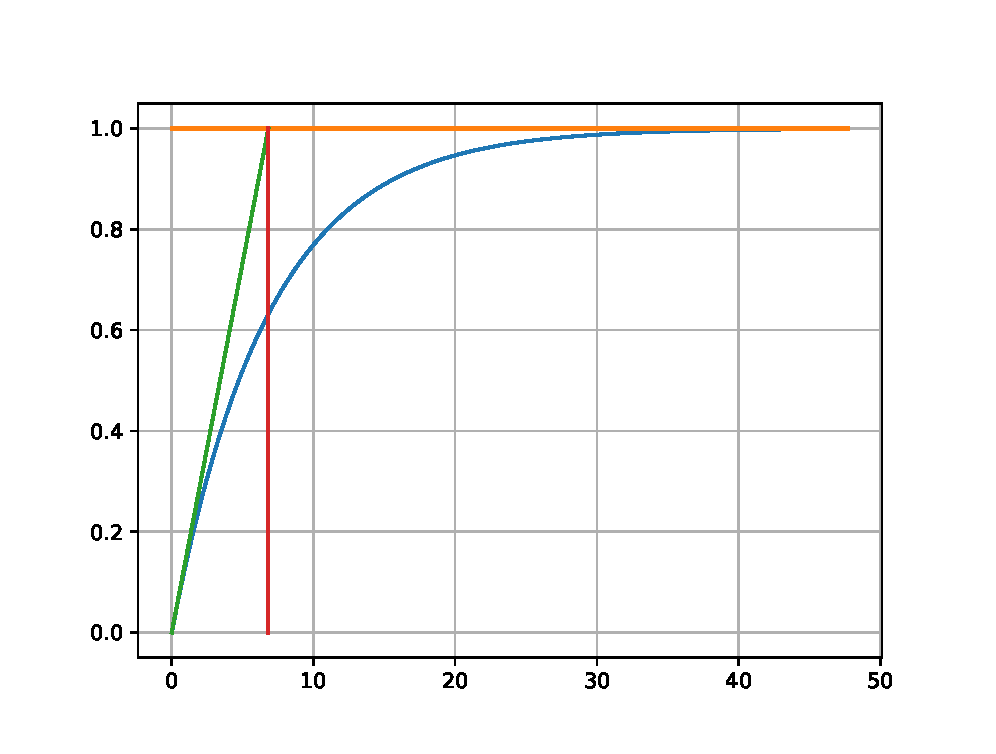
\includegraphics[width=0.7\linewidth]{img/motoreduc_courbe_cor}
\end{center}

\subsection{Diravi}

\paragraph{Question 1:}

\begin{figure}[!h]
\begin{center}
\begin{tikzpicture}[scale=0.8, every node/.style={scale=0.8}]
\sbEntree{E}
\sbBloc{ka}{$K_a$}{E}
\sbRelier[$\alpha_{vol}$]{E}{ka}
\sbComp{comp}{ka}                
\sbRelier[$\alpha$]{ka}{comp}
\sbBloc{reg}{$K_b$}{comp}  
\sbRelier[$\epsilon$]{comp}{reg}
\sbBloc{k}{$k$}{reg}  
\sbRelier[$X(p)$]{reg}{k}
\sbComp{compdeux}{k}
\sbRelier[$Q(p)$]{k}{compdeux}
\sbDecaleNoeudx[8]{compdeux}{re}
\sbBloc{res}{$\dfrac{1}{S.p}$}{re}      
\sbRelier[$\epsilon_Q$]{compdeux}{res}
\sbDecaleNoeudx[15]{res}{r}
\sbSortie{S}{r}
\sbRelier[$Y(p)$]{res}{S}
\sbDecaleNoeudy[5]{S}{U}
\sbDecaleNoeudx[-7]{U}{V}
\sbBlocr{cap}{$M.p^2$}{V}        
\sbRelieryx{res-S}{cap}
\sbBlocr{pis}{$\dfrac{1}{S}$}{cap}
\sbRelier[$F(p)$]{cap}{pis}
\sbBlocr{beta}{$\dfrac{V.\beta.p}{2}$}{pis}
\sbRelier[$\Delta_p(p)$]{pis}{beta}
\sbDecaleNoeudx[-10]{beta}{c}
\sbCompSum{comptrois}{c}{}{+}{}{+}
\sbRelier[$Q_c(p)$]{beta}{comptrois}
\sbRelierxy[$M_v$]{comptrois}{compdeux}
\sbDecaleNoeudy[4]{pis}{G}
\sbDecaleNoeudx[-2]{G}{fe}
\sbBlocr{f}{$f$}{fe}
\sbRelierxy[$Q_p(p)$]{f}{comptrois}
\sbRelieryx{pis-beta}{f}
\sbDecaleNoeudy[13]{S}{W}
\sbDecaleNoeudx[-8]{W}{X}
\sbBlocr[5]{kc}{$K_c$}{X}        
\sbRelieryx{res-S}{kc}
\sbBlocr[5]{kd}{$K_d$}{kc} 
\sbRelier[$\alpha_{pignon}$]{kc}{kd}  
\sbRelierxy[$\alpha'$]{kd}{comp}
\end{tikzpicture}
\end{center}
 \caption{Schéma bloc}
 \label{blocs1}
\end{figure}

\paragraph{Question 2:} 

$FTBO(p)=\dfrac{\alpha'(p)}{\epsilon(p)}=K_b.k.K_c.K_d.H(p)$

$H(p)=\dfrac{\dfrac{1}{S.p}}{1+\dfrac{1}{S.p}.M.p^2.\dfrac{1}{S}.\left(f+\dfrac{V.\beta.p}{2}\right)}$

$FTBO(p)=\dfrac{\dfrac{K_b.k.K_c.K_d.}{S}}{p.\left(1+\dfrac{M.f}{S^2}.p+\dfrac{V.\beta.M}{2.S^2}.p^2\right)}$

$FTBF(p)=\dfrac{K_a.K_b.k.H(p)}{1+FTBO(p)}$

$FTBF(p)=\dfrac{\dfrac{K_a}{K_c.K_d}}{1+\dfrac{S}{K_b.k.K_c.K_d}.p+\dfrac{M.f}{S.K_b.k.K_c.K_d}.p^2+\dfrac{M.V.\beta}{2.S.K_b.k.K_c.K_d}.p^3}$

\paragraph{Question 3:}

La FTBF est de classe 0 et d'ordre 3.


\paragraph{Question 4:} 

\begin{itemize}
 \item $K_a=\dfrac{34}{57}$,
 \item $K_b=0,04mm.\degree^{-1}=0,04.10^{-3}.\frac{180}{\pi}m.rad^{-1}$,
 \item $K_c=\dfrac{1}{500}tr.mm^{-1}=\dfrac{2.\pi.10^3}{500}rad.m^{-1}$,
 \item $K_d=K_a$,
 \item $k=0,24m^3.s^{-1}.mm^{-1}=0,24.10^3m^3.s^{-1}.m^{-1}$,
 \item $S=3000mm^2=3000.10^{-6}m^2$,
 \item $M=500kg$,
 \item $f=6.dm^3.min^{-1}.MPa^{-1}=6.10^{-3}.\frac{1}{60}.10^{-6}m^5.s^{-1}.N^{-1}$,
 \item $\dfrac{V.\beta}{2}=2*10^{-5}.10^{-3}.10^{-6}m^5.N^{-1}$
\end{itemize}

\paragraph{Question 5:}

On constate que $\dfrac{V.\beta}{2}$ est négligeable devant $f$, donc on peut négliger le terme de degré 3.

$K=\frac{K_a}{K_c.K_d}$

$\omega_0=\sqrt{\frac{S.K_b.k.K_c.K_d}{M.f}}$

$\xi=\frac{S.\sqrt{S}}{2.\sqrt{K_b.k.K_c.K_d.M.f}}$

$\omega_0=\sqrt{\frac{3000.10^{-6}.0,04.10^{-3}.\frac{180}{\pi}.0,24.10^3.\frac{2.\pi.10^3}{500}.\frac{34}{57}}{500.6.10^{-3}.\frac{1}{60}.10^{-6}}}=\sqrt{\frac{3.10^{-3}.4.10^{-4}.\frac{18}{\pi}.24.10^1.4.\pi.\frac{34}{57}}{5.6.10^{-1}.\frac{1}{6}.10^{-7}}}
=12.6.10.\sqrt{\frac{4.34}{57.5}}\approx12.6.10.\sqrt{\frac{4.36}{285}}\approx2.6.12.6.10.\sqrt{\frac{1}{25*12}}\approx\frac{6.12.6.10}{5}.\sqrt{\frac{1}{3}}\approx\frac{6.12.6.10}{5.1,7}\approx\frac{6.12.6.10}{5.1,7}\approx\frac{864}{1,7}\approx500rad^{-1}.$

$\xi=\frac{3000.10^{-6}.\sqrt{3000.10^{-6}}}{2.\sqrt{0,04.10^{-3}.\frac{180}{\pi}.0,24.10^3.\frac{2.\pi.10^3}{500}.\frac{34}{57}.500.6.10^{-3}.\frac{1}{60}.10^{-6}}}=\frac{3000.10^{-8}.\sqrt{30}}{2.\sqrt{4.10^{-4}.18.24.10.4.\frac{34}{57}.5.10^{-2}.10^{-6}}}\approx\frac{3000.10^{-8}.\sqrt{30}}{480.10^{-6}.\sqrt{12.\frac{17}{57}}}\approx\frac{3.\sqrt{10}}{48}\approx\frac{9}{48}\approx0,2$

$K=\frac{\frac{34}{57}}{\frac{2.\pi.10^3}{500}.\frac{34}{57}}=\frac{1}{4.\pi}\approx0,08$

Valeurs sans approximations intermédiaires:
$\omega_0=497,37rad.s^{-1}$, $\xi=0,18$.

\paragraph{Question 6:}

\begin{center}
 \includegraphics[width=0.7\linewidth]{img/diravi_temp}
\end{center}

$t_{R,5\%}=\dfrac{ln(20)}{\xi.\omega_0}=0.033s$

$D\%=100.e^{-\xi.\dfrac{\pi}{\sqrt{1-\xi^2}}}=56\%$.

\subsection{Centre usinage grande vitesse}

\paragraph{Question 1:} On mesure le temps de réponse à 5\% à 0,45ms. Ainsi, la fonction de transfert du premier ordre est la suivante:

$\dfrac{C(p)}{C_{ref}(p)}=\dfrac{\dfrac{2,91}{3}}{1+0,15.10^{-3}.p}=\dfrac{0,97}{1+0,15.10^{-3}.p}$

\paragraph{Question 2:} Sur le graphique, le retard se mesure à $r=0,25ms$.

$\dfrac{C(p)}{C_{ref}(p)}=\dfrac{0,97}{1+0,15.10^{-3}.p}.e^{-r.p}=\dfrac{0,97}{1+0,15.10^{-3}.p}.e^{-0,25.10^{-3}.p}$

\paragraph{Question 3:} En remplaçant $e^{-r.p}$ par son développement limité à l'ordre 1: $\dfrac{1}{1+r.p}$

$\dfrac{C(p)}{C_{ref}(p)}=\dfrac{0,97}{1+0,15.10^{-3}.p}.\dfrac{1}{1+r.p}=\dfrac{0,97}{(1+0,00025.p)(1+0,00015.p)}$

\subsection{Système de traite automatique des vaches}

\paragraph{Questions 1 et 2:} 

$H(p)=\dfrac{\frac{\Phi_p.r}{2.K_e}}{1+\frac{R.r^2.\Phi_p^2.M_{eq}}{4.K_i.K_e}.p+\frac{L.r^2.\Phi_p^2.M_{eq}}{4.K_i.K_e}.p^2}$

$G=\dfrac{\Phi_p.r}{2.K_e}=0,59$

$\omega_0=\sqrt{\frac{4.K_i.K_e}{L.r^2.\Phi_p^2.M_{eq}}}=\frac{2}{r.\Phi_p}.\sqrt{\frac{K_i.K_e}{L.M_{eq}}}=3,27rad.s^{-1}$

$\xi=\frac{R.r.\Phi_p}{4}.\sqrt{\frac{M_{eq}}{L.K_i.K_e}}=16,14$

$\xi$ est plus grand que 1, il existe donc deux racines réelles $\tau_1$ et $\tau_2$.

$\tau_1=\frac{1}{\omega_0.(\xi-\sqrt{\xi^2-1}))}=10s$

$\tau_2=\frac{1}{\omega_0.(\xi+\sqrt{\xi^2-1}))}=0,01s$

On peut négliger l'effet de $\tau_2$ sur la réponse du système, ainsi on peut écrire:

$H(p)=\frac{G}{1+\tau_1.p}$.

\paragraph{Question 3:}

$FTBO(p)=\frac{X_m(p)}{\epsilon (p)}=\frac{C(p).G.K_c}{p(1+\tau_1.p)}=\frac{G.K_c}{p(1+\tau_1.p)}$

\paragraph{Question 4:}

$FTBF(p)=\frac{1}{1+\frac{1}{K_c.G}.p+\frac{\tau_1}{K_c.G}.p^2}$, avec:

\begin{itemize}
 \item $\omega_0=\sqrt{\frac{K_c.G}{\tau_1}}=1,9rad.s^{-1}$,
 \item $\xi=\frac{1}{2.\sqrt{K_c.G.\tau_1}}=0,025$
\end{itemize}

\subsection{Transmission Vario-Fendt}

\paragraph{Questions 1:}

$U(p)=R.I(p)+k_e.p.\theta(p)$, $Je.p^2.\theta(p)=k_a.I(p)$

$M(p)=\frac{\frac{1}{k_e}}{p.(1+\frac{R.Je}{k_e.k_a}.p)}$

\begin{itemize}
 \item $K_m=\frac{1}{k_e}=20rad.s^{-1}.V^{-1}$
 \item $\tau_m=\frac{R.Je}{k_e.k_a}=0,5s$
\end{itemize}

\paragraph{Questions 2:}

$T(p)=\frac{U_r(p)}{\epsilon(p)}=K_c.K_r.M(p)=\frac{K_c.K_r.K_m}{p.(1+\tau_m.p)}$

$K_{BO}=K_c.K_r.K_m$

\paragraph{Questions 3:}

$F(p)=\frac{\frac{K_c.K_m}{p.(1+\tau_m.p)}}{1+\frac{K_c.K_r.K_m}{P.(1+\tau_m.p)}}=\frac{\frac{1}{K_r}}{1+\frac{1}{K_c.K_r.K_m}.p+\frac{\tau_m}{K_c.K_r.K_m}.p^2}$

\begin{itemize}
 \item $K_{BF}=\frac{1}{K_r}$,
 \item $\omega_0=\sqrt{\frac{K_c.K_r.K_m}{\tau_m}}$,
 \item $\xi=\frac{1}{2.\sqrt{K_c.K_r.K_m.\tau_m}}$.
\end{itemize}

\paragraph{Questions 4:}

Le temps de réponse le plus rapide sans dépassement implique $\xi=1$.

Ainsi, $K_{BO}=\frac{1}{4.\tau_m}=0,5s^{-1}$.

Donc, $K_c=0,0125V$.

\paragraph{Questions 5:}

Si $\xi=1$, alors le polynôme du dénominateur compte deux racines doubles, avec  $T=\frac{1}{\omega_0}$.

Ainsi, $T=1s$.

\paragraph{Questions 6:}

Ici, $t_{R,5\%}=4,75s>1s$, le système ne respecte pas le cahier des charges.

\paragraph{Questions 7:}

$\theta(p)=M(p).\left[U(p)-\theta(p).k_p\right]$

$\frac{\theta(p)}{U(p)}=\frac{M(p)}{1+M(p).k_p}=\frac{\frac{K_m}{1+K_m.k}}{p.(1+\frac{\tau_m}{1+K_m.k}.p)}$

$K'_m=\frac{K_m}{1+k.K_m}$

$\tau'_m=\frac{\tau_m}{1+k.K_m}$

Le temps de réponse doit être dois fois plus court, donc $\tau'_m=\frac{\tau_m}{10}$, donc $1+k.K_m=10$, donc $k=\frac{9}{K_m}=0,45V.rad^{-1}.s$.

$K'_m=2rad.s^{-1}.V^{-1}$

$K_{BO}=5$, $K_c=1.25$, $K_{BF}=0,5rad.V^{-1}$, $T=0,1s$

\paragraph{Questions 8:}

$K=\frac{\frac{\pi}{4}}{12}=6,545.10^{-2}rad.V^{-1}$

$K=K_{BF}.K_p$ et $K_p=p_p.\frac{b}{a.d}$, donc  $a=\frac{K_{BF}.p_p.200}{d.K+K_{BF}.p_p}$

Donc, $a=90mm$ et $b=110mm$.

\paragraph{Questions 9:}

Si $T_p<0,2s$, alors $\frac{(a+b).S.c}{a.d.K_d}<0,2$, donc $S<\frac{0,2.a.d.K_d}{200.c}$, ainsi $S=675mm^2$, donc $D=29,32mm$.

\end{document}
